\documentclass{standalone}
\usepackage{amssymb} 
\usepackage{tikz} 
\usetikzlibrary{positioning}

\tikzset{set/.style={draw,circle,inner sep=0pt,align=center}}

\begin{document}

\[
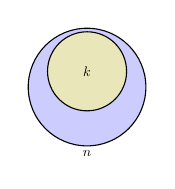
\begin{tikzpicture}[baseline, scale=0.5,transform shape]
\node[set,fill=blue!20,text width=3cm,label={[below=85pt of rea]$n$}] 
  (nat) at (0,-0.4)  (rea) {};
  \node[set,fill=olive!20,text width=2cm] (nat) at (0,0) {$k$};

\end{tikzpicture}
=
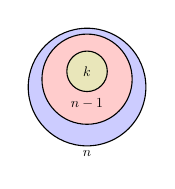
\begin{tikzpicture}[baseline, scale=0.5,transform shape]
\node[set,fill=blue!20,text width=3cm,label={[below=85pt of rea]$n$}] 
  (nat) at (0,-0.4)  (rea) {};
  \node[set,fill=red!20,text width=2.3cm,label={[below=43pt of int]$n-1$}] 
  (int) at (0,-0.2)  {};
\node[set,fill=olive!20,text width=1cm] (nat) at (0,0) {$k$};

\end{tikzpicture}

+

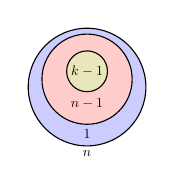
\begin{tikzpicture}[baseline, scale=0.5,transform shape]
\node[set,fill=blue!20,text width=3cm,label={[below=85pt of rea]$n$}] 
  (nat) at (0,-0.4)  (rea) {};
  \node[set,fill=red!20,text width=2.3cm,label={[below=43pt of int]$n-1$}] 
  (int) at (0,-0.2)  {};
\node[set,fill=olive!20,text width=1cm] (nat) at (0,0) {$k-1$};
\node[label={[below=42pt of int]$1$}] (nat) at (0,0) {};

\end{tikzpicture}

\]
\end{document}
